\chapter{Músculos e articulações}\label{ch:g10:muscles-and-joints}

Um jogador de futebol firma o pé, gira e cai segurando o joelho. O
diagnóstico, uma hora depois: um \omterm{def:g10:muscles-and-joints:joint}{ligamento} rompido. Nada nos ossos está
quebrado, nenhum músculo falhou; uma tira de tecido de alguns
centímetros, cuja função era manter dois ossos alinhados, cedeu sob uma
torção para a qual ela nunca foi construída. Para entender o que se
rompeu, e por que o joelho vai precisar de meses para se recuperar,
precisamos saber do que é feita uma \omterm{def:g10:muscles-and-joints:joint}{articulação}, como os músculos
puxam nela, e que forças a atravessam quando um corpo de setenta
quilogramas aterrissa sobre uma perna só.

\section{A articulação}

\begin{definition}[Articulação]\label{def:g10:muscles-and-joints:joint}
Uma \emph{articulação}\index{articulação} é o lugar onde dois ossos se
encontram. Numa articulação móvel como o joelho, o quadril, o ombro ou
o cotovelo, as extremidades dos ossos são revestidas por uma camada de
\emph{cartilagem}\index{cartilagem} lisa, de alguns milímetros de
espessura, e encerradas num saco vedado, a \emph{cápsula}, cujo
revestimento secreta o \emph{líquido sinovial} que lubrifica as
superfícies. Faixas de tecido resistente, os
\emph{ligamentos}\index{ligamento}, vão de osso a osso através da
articulação e limitam os movimentos dela aos previstos. No joelho, dois
crescentes de cartilagem, os \emph{meniscos}, ficam entre os ossos e
distribuem a carga.
\end{definition}

\begin{omfigure}
\begin{tikzpicture}
  \node[anchor=south west, inner sep=0] (img) at (0,0)
    {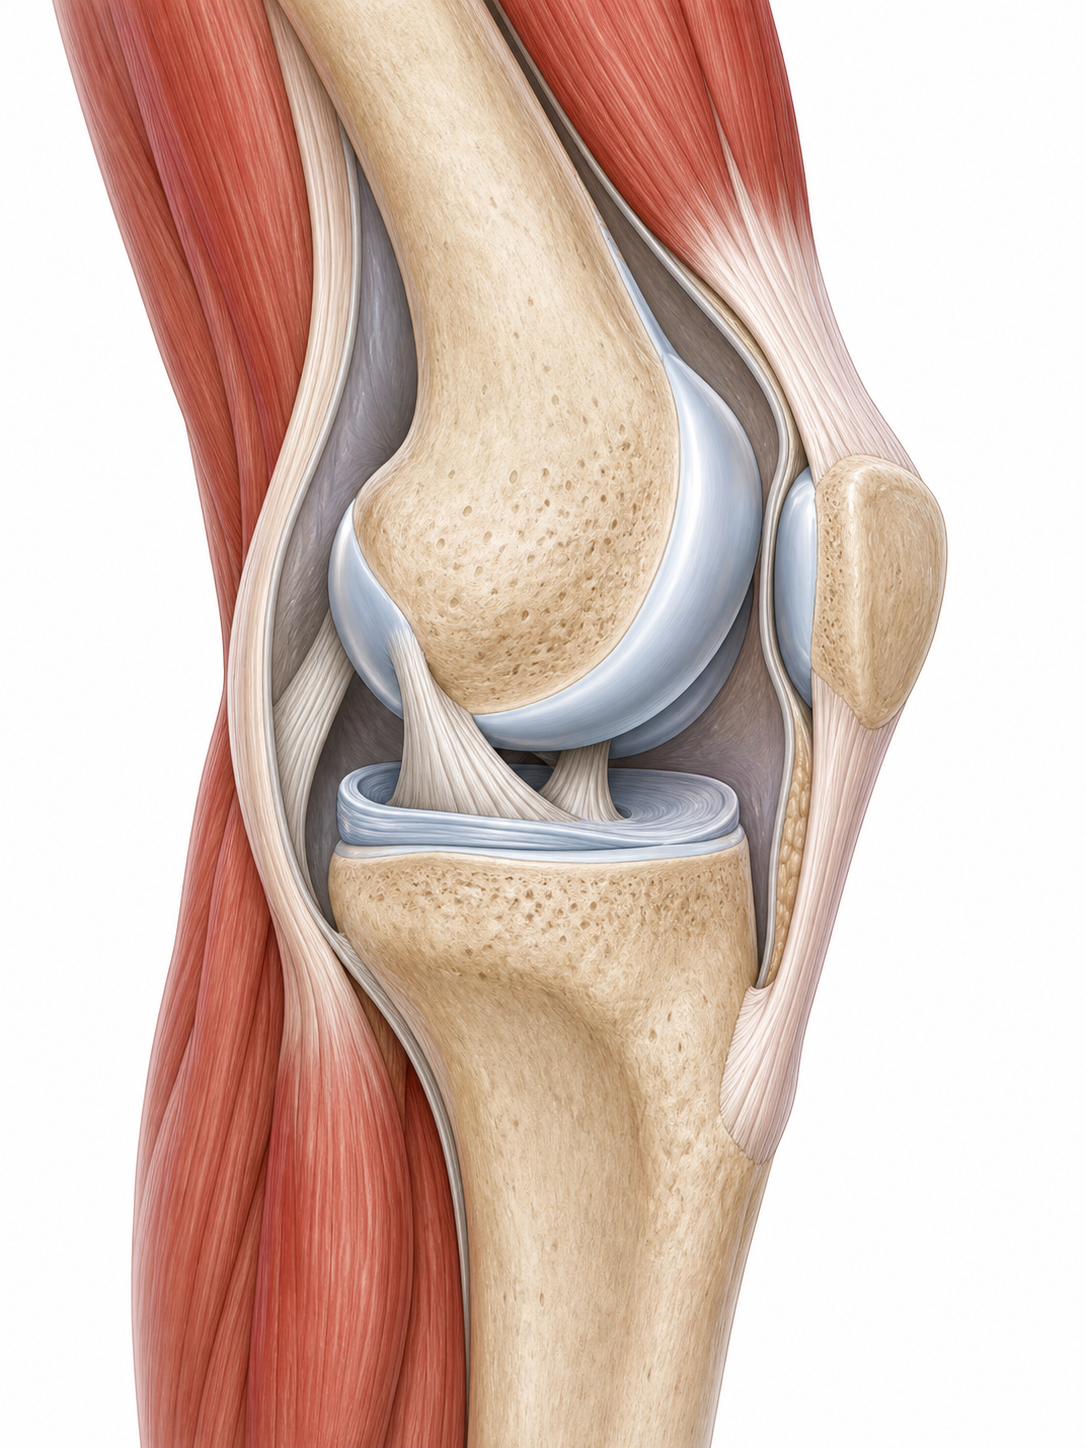
\includegraphics[width=0.4\linewidth]{images/book2/ai/fig-knee-cutaway.png}};
  \begin{scope}[x={(img.south east)}, y={(img.north west)},
      every node/.style={font=\small}]
    \draw[omDef, thick] (0.50,0.86) -- (1.05,0.90) node[right] {fêmur};
    \draw[omDef, thick] (0.76,0.74) -- (1.05,0.74) node[right] {tendão do quadríceps};
    \draw[omDef, thick] (0.82,0.58) -- (1.05,0.58) node[right] {patela};
    \draw[omDef, thick] (0.50,0.20) -- (1.05,0.14) node[right] {tíbia};
    \draw[omDef, thick] (0.34,0.60) -- (-0.05,0.64) node[left] {cartilagem};
    \draw[omDef, thick] (0.50,0.50) -- (-0.05,0.50) node[left] {ligamento};
    \draw[omDef, thick] (0.40,0.44) -- (-0.05,0.36) node[left] {menisco};
  \end{scope}
\end{tikzpicture}

{\small O joelho em corte: o fêmur em cima, a tíbia embaixo, a patela
(rótula) à frente, no \omterm{def:g10:muscles-and-joints:muscle}{tendão} do músculo da coxa; a \omterm{def:g10:muscles-and-joints:joint}{cartilagem} nas
extremidades dos ossos, o menisco entre elas, os \omterm{def:g10:muscles-and-joints:joint}{ligamentos} segurando
os ossos juntos.}
\end{omfigure}

\begin{proposition}[Para que serve cada parte]\label{prop:g10:muscles-and-joints:parts}
A \omterm{def:g10:muscles-and-joints:joint}{cartilagem} e o líquido sinovial fazem as superfícies deslizarem com
menos atrito que gelo sobre gelo; os meniscos distribuem uma carga que
de outro modo se concentraria em alguns milímetros quadrados; os
\omterm{def:g10:muscles-and-joints:joint}{ligamentos} permitem que o joelho dobre e estique, mas resistem à
torção e à flexão lateral; a cápsula mantém o líquido dentro. Cada
parte tem a falha própria dela: a \omterm{def:g10:muscles-and-joints:joint}{cartilagem} se desgasta (a artrose),
um menisco se rompe numa torção com o joelho dobrado, um \omterm{def:g10:muscles-and-joints:joint}{ligamento}
sofre entorse ou se rompe quando a \omterm{def:g10:muscles-and-joints:joint}{articulação} é forçada além da
amplitude dela.
\end{proposition}
\admitted

\begin{example}[Entorse, ruptura, luxação]\label{ex:g10:muscles-and-joints:injuries}
Torça o tornozelo num meio-fio: os \omterm{def:g10:muscles-and-joints:joint}{ligamentos} do lado de fora são
esticados além do limite deles --- é uma \emph{entorse}; a \omterm{def:g10:muscles-and-joints:joint}{articulação}
incha à medida que a cápsula sangra e o líquido se acumula. Puxe com
força um isquiotibial frio: algumas fibras dele se rompem --- é uma
\emph{ruptura} muscular. Caia sobre o braço estendido: a cabeça do
úmero pode sair da cavidade dela --- é uma \emph{luxação}, com os
\omterm{def:g10:muscles-and-joints:joint}{ligamentos} e a cápsula esticados ou rompidos no processo. Nenhuma
dessas coisas é um osso quebrado; todas podem levar mais tempo para
curar do que ele.
\end{example}

\section{Os músculos puxam, aos pares}

\begin{definition}[Músculo esquelético e tendão]\label{def:g10:muscles-and-joints:muscle}
Um \emph{músculo esquelético}\index{músculo esquelético} é um órgão
feito de milhares de \omterm{def:g10:cells-common-unit:cell}{células} compridas, as \emph{fibras musculares},
reunidas em feixes; cada fibra encurta quando estimulada por um nervo.
Nas duas extremidades o músculo se afina num
\emph{tendão}\index{tendão}, um cordão de tecido não contrátil preso ao
osso. Um músculo só consegue \emph{puxar}, encurtando, e apenas ao
longo do próprio comprimento: ele move uma \omterm{def:g10:muscles-and-joints:joint}{articulação} puxando o osso
que está do outro lado dela.
\end{definition}

\begin{proposition}[Pares antagonistas]\label{prop:g10:muscles-and-joints:antagonists}
Como um músculo não consegue empurrar, todo movimento de uma
\omterm{def:g10:muscles-and-joints:joint}{articulação} exige dois músculos ou dois grupos trabalhando em oposição:
um \emph{flexor} que dobra a \omterm{def:g10:muscles-and-joints:joint}{articulação} e um \emph{extensor} que a
estica. Quando um se contrai, o outro relaxa e é esticado; para manter
uma posição, os dois se contraem juntos. O bíceps flexiona o cotovelo e
o tríceps o estende; o quadríceps, na frente da coxa, estende o joelho,
e os isquiotibiais, atrás dele, o flexionam.
\end{proposition}
\admitted

\begin{omfigure}
\begin{tikzpicture}[>=Stealth, font=\small, line cap=round]
  % upper arm (humerus) horizontal, forearm angled
  \draw[line width=7pt, gray!45] (0,0) -- (5,0);         % humerus
  \draw[line width=6pt, gray!45] (5,0) -- (8.6,2.0);     % forearm
  \fill[gray!60] (5,0) circle (0.28);
  \node[anchor=north] at (2.5,-0.25) {úmero};
  \node[anchor=north west] at (7.2,1.1) {antebraço};
  \node[anchor=west] at (5.5,-0.5) {cotovelo};
  % biceps: from shoulder region above humerus to forearm just past elbow
  \draw[line width=9pt, omThm!60] (0.6,0.6) .. controls (3,1.4) .. (5.35,0.9);
  \draw[thick, omThm!80!black] (5.35,0.9) -- (5.65,0.45);   % tendon
  \node[omThm!80!black, anchor=south] at (3,1.3) {bíceps (flexor): contrai-se};
  % triceps: below humerus to the back of the forearm
  \draw[line width=7pt, omDef!50] (0.6,-0.9) .. controls (3,-1.6) .. (4.9,-1.0);
  \draw[thick, omDef!80!black] (4.9,-1.0) -- (5.25,-0.4);
  \node[omDef!80!black, anchor=north] at (3,-1.65) {tríceps (extensor): relaxa, é esticado};
  \draw[->, thick] (8.6,2.0) to[bend right=20] (8.0,3.0);
  \node[anchor=south] at (8.3,3.05) {flexão};
  \draw[->, thick, omThm!80!black] (5.65,0.45) -- (5.2,0.75);
\end{tikzpicture}

{\small Um par antagonista no cotovelo. O bíceps, preso ao antebraço
logo depois da \omterm{def:g10:muscles-and-joints:joint}{articulação}, encurta e dobra o cotovelo; o tríceps,
preso atrás da \omterm{def:g10:muscles-and-joints:joint}{articulação}, relaxa e é esticado. Inverta os papéis para
esticar o braço.}
\end{omfigure}

\begin{proposition}[Alavancas e forças]\label{prop:g10:muscles-and-joints:lever}
Um osso que gira numa \omterm{def:g10:muscles-and-joints:joint}{articulação} é uma alavanca. O \omterm{def:g10:muscles-and-joints:muscle}{tendão} do músculo
se prende a uma distância curta $d$ do pivô, enquanto a carga age a uma
distância maior $D$; para o equilíbrio, o músculo precisa puxar com uma
força
\[
F_{\text{músculo}} = F_{\text{carga}} \times \frac{D}{d},
\]
várias vezes maior que a carga. O arranjo troca força por velocidade e
amplitude: um encurtamento pequeno do músculo produz um movimento
grande e rápido da mão ou do pé, ao preço de forças grandes no \omterm{def:g10:muscles-and-joints:muscle}{tendão} e
na \omterm{def:g10:muscles-and-joints:joint}{articulação}.
\end{proposition}
\admitted

\begin{example}[Segurar uma sacola]\label{ex:g10:muscles-and-joints:bag}
Uma sacola de \qty{5}{kg} (peso de \qty{49}{N}) pende da mão, a
\qty{35}{cm} do cotovelo; o \omterm{def:g10:muscles-and-joints:muscle}{tendão} do bíceps se prende a \qty{5}{cm}
dele. O bíceps puxa com $49 \times 35/5 = \qty{343}{N}$ --- sete vezes
a carga, o peso de \qty{35}{kg} --- e a \omterm{def:g10:muscles-and-joints:joint}{articulação} do cotovelo é
comprimida com cerca de \qty{300}{N}. Os músculos, os tendões e a
\omterm{def:g10:muscles-and-joints:joint}{cartilagem} são construídos para essas forças; o que os danifica é uma
força súbita na direção errada, ou uma carga repetida além do que o
tecido consegue reparar.
\end{example}

\begin{omfigure}
\begin{tikzpicture}[>=Stealth, font=\small]
  \draw[line width=6pt, gray!45] (0,0) -- (7,0);
  \fill[gray!70] (0,0) circle (0.25);
  \node[anchor=north] at (0,-0.35) {cotovelo (pivô)};
  \draw[->, very thick, omThm] (1,0.15) -- (1,2.2) node[above] {$F_{\text{músculo}}$};
  \draw[->, very thick, omDef] (7,-0.15) -- (7,-1.6) node[below] {$F_{\text{carga}} = \qty{49}{N}$};
  \draw[<->] (0,0.9) -- (1,0.9) node[midway, above, xshift=-4mm] {$d = \qty{5}{cm}$};
  \draw[<->] (0,-1.25) -- (7,-1.25) node[midway, below] {$D = \qty{35}{cm}$};
\end{tikzpicture}

{\small O antebraço como alavanca: o bíceps puxa perto do pivô, a carga
pende longe dele. $F_{\text{músculo}} \times d =
F_{\text{carga}} \times D$, de modo que a força do músculo é $D/d = 7$
vezes a carga.}
\end{omfigure}

\section{Por dentro do músculo}

\begin{proposition}[Estrutura de uma fibra muscular]\label{prop:g10:muscles-and-joints:fibre}
Uma fibra muscular é uma única \omterm{def:g10:cells-common-unit:cell}{célula} gigante, de
\num{10}--\qty{100}{\micro m} de largura e até vários centímetros de
comprimento, com muitos \omterm{def:g10:cells-common-unit:organelle}{núcleos}. Ela é abarrotada de
\emph{miofibrilas} paralelas, cada uma uma cadeia de unidades
repetidas em que dois tipos de filamento de \omterm{def:g10:chemistry-of-life:families}{proteína}, grossos e finos,
se interpenetram. A contração é o deslizamento dos filamentos finos
entre os grossos, movido por ATP: cada unidade encurta uma fração, a
miofibrila encurta a soma delas, e a fibra encurta junto. As
\omterm{def:g10:cells-common-unit:organelle}{mitocôndrias} entre as miofibrilas fornecem o ATP; uma terminação
nervosa em cada fibra dá a ordem.
\end{proposition}
\admitted

\begin{omfigure}
\begin{tikzpicture}[font=\small, >=Stealth]
  \tikzset{lvl/.style={draw, rounded corners, thick, align=center, minimum height=1.1cm}}
  \node[lvl, fill=omThm!12, text width=2.1cm] (m) at (0,0) {músculo\\ (órgão)};
  \node[lvl, fill=omThm!12, text width=2.1cm] (b) at (3.0,0) {feixe de\\ fibras};
  \node[lvl, fill=omProp!15, text width=2.1cm] (f) at (6.0,0) {fibra muscular\\ (uma célula)};
  \node[lvl, fill=omDef!12, text width=2.1cm] (my) at (9.0,0) {miofibrila};
  \node[lvl, fill=omMeth!15, text width=2.1cm] (fi) at (12.0,0) {filamentos\\ grossos e finos};
  \foreach \a/\b in {m/b, b/f, f/my, my/fi} \draw[->] (\a) -- (\b);
  \node[anchor=north, font=\scriptsize] at (m.south) {centímetros};
  \node[anchor=north, font=\scriptsize] at (b.south) {milímetro};
  \node[anchor=north, font=\scriptsize] at (f.south) {\qty{50}{\micro m} de largura};
  \node[anchor=north, font=\scriptsize] at (my.south) {\qty{1}{\micro m} de largura};
  \node[anchor=north, font=\scriptsize] at (fi.south) {\qty{10}{nm}};
\end{tikzpicture}

{\small Do músculo inteiro até as moléculas que o encurtam: cinco
níveis de organização, cada um um feixe do seguinte. O deslizamento dos
filamentos uns sobre os outros, repetido em cada unidade, é a
contração.}
\end{omfigure}

\begin{definition}[Tipos de fibra]\label{def:g10:muscles-and-joints:types}
As \omterm{def:g10:muscles-and-joints:muscle}{fibras musculares} vêm em dois tipos principais. As
\emph{fibras lentas} se contraem devagar e fracamente, mas sem se
cansar: ricas em \omterm{def:g10:cells-common-unit:organelle}{mitocôndrias} e em capilares, avermelhadas por uma
\omterm{def:g10:chemistry-of-life:families}{proteína} que armazena oxigênio, elas funcionam com a respiração e
predominam nos músculos posturais e nos atletas de resistência. As
\emph{fibras rápidas} se contraem depressa e com força, mas se cansam
em menos de um minuto: mais pobres em \omterm{def:g10:cells-common-unit:organelle}{mitocôndrias}, mais pálidas, elas
contam com a reserva de fosfato e com a \omterm{def:g10:cell-metabolism:fermentation}{fermentação} e predominam nos
velocistas. A proporção num dado músculo é em grande parte herdada; o
treinamento muda o tamanho e o equipamento das fibras mais do que o
número delas.
\end{definition}

\begin{example}[Ler uma biópsia muscular]\label{ex:g10:muscles-and-joints:biopsy}
Uma coloração para as \omterm{def:g10:cell-metabolism:metabolism}{enzimas} das \omterm{def:g10:cells-common-unit:organelle}{mitocôndrias} numa fatia fina de
músculo da coxa mostra um mosaico: fibras escuras (lentas) e fibras
pálidas (rápidas). A amostra de um maratonista tem 80\% de escuras; a
de um velocista, 30\%; a de uma pessoa não treinada, cerca de metade e
metade. A mesma coloração no mesmo corredor depois de um ano de treino
de velocidade mostra as fibras pálidas aumentadas, mas não mais
numerosas.
\end{example}

\section{Fadiga, dano, reparo}

\begin{proposition}[Limites do músculo]\label{prop:g10:muscles-and-joints:limits}
Um músculo falha de três maneiras distintas. A \emph{fadiga}: a força
diminui quando o fornecimento de ATP não consegue acompanhar --- em
menos de um minuto nas fibras rápidas, ao longo de horas nas lentas ---
e se recupera com o descanso. A \emph{cãibra}: uma contração súbita,
sustentada e involuntária, muitas vezes por desidratação ou perda de
sal. A \emph{lesão}: fibras rompidas por uma força que ultrapassa a
resistência delas, tipicamente quando o músculo está frio, cansado ou
sendo esticado enquanto se contrai. As fibras se reparam ao longo de
semanas a partir de \omterm{def:g10:cells-common-unit:cell}{células} de reserva do músculo; um \omterm{def:g10:muscles-and-joints:muscle}{tendão} ou um
\omterm{def:g10:muscles-and-joints:joint}{ligamento}, mal irrigados de sangue, se reparam ao longo de meses.
\end{proposition}
\admitted

\begin{method}[Analisar uma lesão musculoesquelética]\label{met:g10:muscles-and-joints:analyse}
\begin{enumerate}
  \item Identifique o movimento que a causou e a direção dele: a
        \omterm{def:g10:muscles-and-joints:joint}{articulação} foi movida dentro da amplitude dela (problema
        muscular) ou além dela (problema de \omterm{def:g10:muscles-and-joints:joint}{ligamento} ou de cápsula)?
  \item Identifique o tecido: as \omterm{def:g10:muscles-and-joints:muscle}{fibras musculares} se rompem (dor no
        ventre do músculo, fraqueza); os \omterm{def:g10:muscles-and-joints:joint}{ligamentos} sofrem entorse
        (dor e inchaço na \omterm{def:g10:muscles-and-joints:joint}{articulação}, instabilidade); os tendões
        inflamam sob carga repetida; a \omterm{def:g10:muscles-and-joints:joint}{cartilagem} se desgasta em
        silêncio ao longo de anos.
  \item Estime a força: use a regra da alavanca; lembre que aterrissar
        ou frear multiplica o peso do corpo várias vezes.
  \item Preveja a recuperação a partir da irrigação sanguínea do
        tecido: músculo em semanas, \omterm{def:g10:muscles-and-joints:joint}{ligamento} e \omterm{def:g10:muscles-and-joints:muscle}{tendão} em meses,
        \omterm{def:g10:muscles-and-joints:joint}{cartilagem} quase nada.
\end{enumerate}
\end{method}

\begin{remark}[Por que o aquecimento funciona]\label{rem:g10:muscles-and-joints:warmup}
Dez minutos de movimento leve elevam a temperatura dos músculos em um
ou dois graus, o que torna as \omterm{def:g10:chemistry-of-life:families}{proteínas} deles mais extensíveis e as
\omterm{def:g10:cell-metabolism:metabolism}{enzimas} deles mais rápidas; ele abre os capilares que vão entregar o
oxigênio do \cref{ch:g10:heart-lungs-effort}, e engrossa a película de
líquido sinovial sobre a \omterm{def:g10:muscles-and-joints:joint}{cartilagem}. Um músculo frio ao qual se pede
uma contração máxima é a causa mais comum de uma ruptura; uma
\omterm{def:g10:muscles-and-joints:joint}{articulação} carregada antes de o líquido dela se espalhar se desgasta
mais depressa.
\end{remark}

\section{Exercícios}

\begin{exercise}[$\star$]\label{exo:g10:muscles-and-joints:1}
Cite as partes de uma \omterm{def:g10:muscles-and-joints:joint}{articulação} móvel e dê o papel de cada uma.
\end{exercise}

\begin{exercise}[$\star$]\label{exo:g10:muscles-and-joints:2}
Qual é a diferença entre um \omterm{def:g10:muscles-and-joints:muscle}{tendão} e um \omterm{def:g10:muscles-and-joints:joint}{ligamento}?
\end{exercise}

\begin{exercise}[$\star$]\label{exo:g10:muscles-and-joints:3}
Por que toda \omterm{def:g10:muscles-and-joints:joint}{articulação} precisa de pelo menos dois músculos para se mover?
\end{exercise}

\begin{exercise}[$\star$]\label{exo:g10:muscles-and-joints:4}
Distinga uma entorse, uma ruptura muscular e uma luxação pelo tecido
envolvido.
\end{exercise}

\begin{exercise}[$\star$]\label{exo:g10:muscles-and-joints:5}
Dê duas diferenças entre as \omterm{def:g10:muscles-and-joints:muscle}{fibras musculares} lentas e as rápidas.
\end{exercise}

\begin{exercise}[$\star\star$]\label{exo:g10:muscles-and-joints:6}
Um halter de \qty{2}{kg} é segurado na mão, a \qty{32}{cm} do cotovelo;
o bíceps se prende a \qty{4}{cm} dele. Calcule a força no bíceps
($g = \qty{9.8}{N/kg}$).
\end{exercise}

\begin{exercise}[$\star\star$]\label{exo:g10:muscles-and-joints:7}
Explique por que o bíceps e o tríceps precisam se contrair os dois para
manter o braço parado contra um empurrão imprevisível.
\end{exercise}

\begin{exercise}[$\star\star$]\label{exo:g10:muscles-and-joints:8}
Uma fibra muscular de \qty{3}{cm} de comprimento encurta 20\% quando se
contrai. De quanto a mão se desloca se o \omterm{def:g10:muscles-and-joints:muscle}{tendão} da fibra se prende a
\qty{5}{cm} do cotovelo e a mão está a \qty{35}{cm} dele?
\end{exercise}

\begin{exercise}[$\star\star$]\label{exo:g10:muscles-and-joints:9}
Por que o ombro, a \omterm{def:g10:muscles-and-joints:joint}{articulação} mais móvel do corpo, é também a que mais
sofre luxações?
\end{exercise}

\begin{exercise}[$\star\star$]\label{exo:g10:muscles-and-joints:10}
A panturrilha de um corredor tem cãibra no fim de uma prova quente.
Proponha duas causas do capítulo e um remédio.
\end{exercise}

\begin{exercise}[$\star\star$]\label{exo:g10:muscles-and-joints:11}
Usando o \cref{ex:g10:muscles-and-joints:biopsy}, explique por que um
velocista que treina para uma maratona melhora menos do que poderia
melhorar uma pessoa não treinada da mesma idade.
\end{exercise}

\begin{exercise}[$\star\star\star$]\label{exo:g10:muscles-and-joints:12}
Na aterrissagem de um salto, o joelho dobra e o \omterm{def:g10:muscles-and-joints:muscle}{tendão} do quadríceps
carrega cerca de quatro vezes o peso do corpo. Para um atleta de
\qty{70}{kg}, calcule essa força. O \omterm{def:g10:muscles-and-joints:muscle}{tendão} tem uma seção transversal de
cerca de \qty{1}{cm^2} e rompe por volta de \qty{100}{N/mm^2}; a que
distância ele está da ruptura?
\end{exercise}

\begin{exercise}[$\star\star\star$]\label{exo:g10:muscles-and-joints:13}
Um \omterm{def:g10:muscles-and-joints:joint}{ligamento} rompido cicatriza ao longo de meses, um músculo rompido ao
longo de semanas, e a \omterm{def:g10:muscles-and-joints:joint}{cartilagem} danificada quase nada. Relacione os
três com a irrigação sanguínea dos tecidos e com as \omterm{def:g10:cells-common-unit:cell}{células} disponíveis
para o reparo.
\end{exercise}

\begin{exercise}[$\star\star\star$]\label{exo:g10:muscles-and-joints:14}
A musculação aumenta os músculos; o alongamento amplia a amplitude de
uma \omterm{def:g10:muscles-and-joints:joint}{articulação}. Que tecido cada um deles muda, e por que nenhum dos
dois muda o número de fibras?
\end{exercise}

\begin{exercise}[$\star\star\star$]\label{exo:g10:muscles-and-joints:15}
A \omterm{def:g10:muscles-and-joints:joint}{cartilagem} do joelho de uma pessoa idosa se desgastou até metade da
espessura. Explique, a partir do capítulo, por que a \omterm{def:g10:muscles-and-joints:joint}{articulação} dói
nas escadas, por que os meniscos importam mais do que antes, e por que
os músculos em volta do joelho fazem parte do tratamento.
\end{exercise}

\section{Problema: as forças num joelho}

\begin{problem}[{Problema de fim de semana --- o joelho de um jogador de
futebol desmontado: a alavanca da perna, a tração do músculo da coxa, o
ligamento que se rompeu, e os números que um tendão carrega a cada
passo}]
\label{pb:g10:muscles-and-joints:1}
Karim, de \qty{70}{kg}, lesionou o joelho ao girar bruscamente com o pé
fincado. Tome $g = \qty{9.8}{N/kg}$. O \omterm{def:g10:muscles-and-joints:muscle}{tendão} do quadríceps se prende à
tíbia a \qty{5}{cm} do pivô do joelho; o empurrão do chão sobre o pé
age a cerca de \qty{20}{cm} dele quando o joelho está bem dobrado, como
numa aterrissagem.

\medskip
\noindent\textbf{Parte I --- De pé e a cada passo.}
\begin{enumerate}
  \item Calcule o peso de Karim.
  \item De pé sobre uma perna com o joelho ligeiramente dobrado, o
        chão empurra o pé para cima com todo o peso dele, agindo a
        \qty{10}{cm} do pivô do joelho. Calcule a força no \omterm{def:g10:muscles-and-joints:muscle}{tendão} do
        quadríceps.
  \item Subindo um degrau, o joelho fica mais dobrado e a força do chão
        age a \qty{20}{cm} do pivô. Calcule de novo a força no \omterm{def:g10:muscles-and-joints:muscle}{tendão}.
  \item Expresse os dois resultados como múltiplos do peso do corpo, e
        explique por que as escadas cansam as coxas.
  \item Que grupo muscular é o antagonista do quadríceps, e o que ele
        está fazendo durante o passo?
\end{enumerate}

\medskip
\noindent\textbf{Parte II --- A aterrissagem.}
\begin{enumerate}[resume]
  \item Ao cair de um cabeceio, o chão empurra com três vezes o peso de
        Karim, a \qty{20}{cm} do pivô. Calcule a força no \omterm{def:g10:muscles-and-joints:muscle}{tendão}.
  \item A seção transversal do \omterm{def:g10:muscles-and-joints:muscle}{tendão} é de \qty{1.2}{cm^2}. Calcule a
        tensão nele, em newtons por milímetro quadrado, e compare com a
        tensão de ruptura de cerca de \qty{100}{N/mm^2}.
  \item As superfícies da \omterm{def:g10:muscles-and-joints:joint}{articulação} são comprimidas uma contra a
        outra por cerca da força do \omterm{def:g10:muscles-and-joints:muscle}{tendão} mais a força do chão.
        Calcule essa carga, depois a pressão sobre a \omterm{def:g10:muscles-and-joints:joint}{cartilagem} se a
        área de contato for de \qty{6}{cm^2} com os meniscos e de
        \qty{1}{cm^2} sem eles.
  \item Deduza por que um joelho que perdeu um menisco desgasta a
        \omterm{def:g10:muscles-and-joints:joint}{cartilagem} mais depressa.
  \item Explique com o que o líquido sinovial contribui durante a
        aterrissagem.
\end{enumerate}

\medskip
\noindent\textbf{Parte III --- A lesão.}
\begin{enumerate}[resume]
  \item O pé de Karim estava fincado e o corpo dele girou: que direção
        de movimento foi imposta ao joelho, e que tecido é construído
        para resistir a ela?
  \item Por que o quadríceps, forte o bastante para puxar com vários
        quilonewtons, não protegeu o \omterm{def:g10:muscles-and-joints:joint}{ligamento}?
  \item O joelho inchou em menos de uma hora. O que o encheu, e que
        parte da \omterm{def:g10:muscles-and-joints:joint}{articulação} foi rompida?
  \item Um exame de imagem mostra o \omterm{def:g10:muscles-and-joints:joint}{ligamento} rompido e um menisco
        lesionado. Usando o
        \cref{met:g10:muscles-and-joints:analyse}, preveja o tempo de
        recuperação de cada um e justifique pela irrigação sanguínea
        deles.
  \item Karim pergunta por que o cirurgião quer fortalecer os
        isquiotibiais dele antes da operação. Responda com a
        \cref{prop:g10:muscles-and-joints:antagonists}.
\end{enumerate}

\medskip
\noindent\textbf{Parte IV --- Cada passo conta.}
\begin{enumerate}[resume]
  \item Karim dá cerca de 8000 passos por dia; metade são sobre a perna
        lesionada. Usando a força da questão 2, quantas vezes por dia o
        \omterm{def:g10:muscles-and-joints:muscle}{tendão} carrega pelo menos essa carga?
  \item Ao longo de um ano, qual é o número total de solicitações?
        Explique por que um \omterm{def:g10:muscles-and-joints:muscle}{tendão} inflamado por uso excessivo (uma
        tendinite) precisa de descanso, e não de força.
  \item Numa partida ele aterrissa de saltos umas 40 vezes. Compare a
        carga total carregada nas aterrissagens (questão 6) com a
        carregada nos passos do dia.
  \item Correr dobra a força do chão em relação a caminhar. Por que os
        médicos recomendam bicicleta e natação em vez de corrida para
        um joelho em recuperação?
  \item Enuncie o resultado: o múltiplo do peso do corpo carregado pelo
        \omterm{def:g10:muscles-and-joints:muscle}{tendão} do quadríceps num degrau e numa aterrissagem, e o único
        tecido do joelho cuja resistência esses números nunca puseram à
        prova --- até o giro.
\end{enumerate}
\end{problem}
